\documentclass{article}

\usepackage{PRIMEarxiv}

\usepackage[utf8]{inputenc}
\usepackage[T1]{fontenc}
\usepackage{hyperref}
\usepackage{url}
\usepackage{booktabs}
\usepackage{amsmath}
\usepackage{amsfonts}
\usepackage{nicefrac}
\usepackage{microtype}
\usepackage{fancyhdr}
\usepackage{graphicx}

\graphicspath{{media/}}

% Header
\pagestyle{fancy}
\thispagestyle{empty}
\rhead{\textit{}}
\fancyhead[LO]{Pluggable kNN Episodic Memory for Deep Q-Learning}

\title{Pluggable kNN Episodic Memory for Deep Q-Learning Agents
in Partially Observable Environments}

\author{
  Anderson G. A. C. Filho,
  Estevan Küster,
  Esthevan F. da Silva,
  João A. T. Laner\\
  Instituto de Informática (INF)\\
  Universidade Federal do Rio Grande do Sul (UFRGS)\\
  Porto Alegre, RS, Brazil\\
  \texttt{anderson.goncalves@ufrgs.br}
}

\date{November 2026}

\begin{document}

\maketitle

\begin{abstract}% TODO: Problem (memory beyond the DTQN context window in POMDPs),
% approach (kNN retrieval over past K/V, as in Memorizing Transformers),
% setup (Passive/Noisy T-Maze, Associative Corridor), main results.
% refs: \cite{esslinger2022dtqn,wu2022memorizing}
\end{abstract}

\keywords{Deep Reinforcement Learning \and Partial Observability \and
Episodic Memory \and Transformers \and k-Nearest Neighbours}

\section{Introduction}
\label{sec:introduction}
% TODO: POMDPs need memory; DTQN only sees the last K observations;
% cues older than the window are lost. Contribution: a pluggable
% kNN episodic memory that extends DTQN's reach without growing K.
% refs: \cite{kaelbling1998pomdp,hausknecht2015drqn,esslinger2022dtqn,wu2022memorizing}

\section{Background}
\label{sec:background}
% TODO: Essentials of RL for a DL audience: MDP/POMDP, Q-learning,
% DQN (replay buffer, target network), DRQN and DTQN.
% refs: \cite{sutton2018rl,kaelbling1998pomdp,mnih2015dqn,vanhasselt2016ddqn,hausknecht2015drqn,esslinger2022dtqn,vaswani2017attention}

\section{Related Work}
\label{sec:related-work}
% TODO: Recurrent and transformer-based agents (DRQN, DTQN, GTrXL),
% memory-augmented transformers (Memorizing Transformers,
% Transformer-XL), episodic memory in RL.
% refs: \cite{hausknecht2015drqn,esslinger2022dtqn,parisotto2020gtrxl,wu2022memorizing,dai2019transformerxl}

\section{Method}
\label{sec:method}
% TODO: Memory population (prefix K/V recomputed under no_grad),
% top-k retrieval per head, gated mix of local and retrieved attention,
% stop-gradient default, per-episode reset; cached variant.
% refs: \cite{wu2022memorizing,esslinger2022dtqn,vaswani2017attention}

\section{Experimental Setup}
\label{sec:experimental-setup}
% TODO: Environments (Passive T-Maze, Noisy T-Maze, Associative
% Corridor; Car Flag and Memory Cards as no-loss checks), baselines
% (DTQN, DRQN), hyperparameters, seeds, metrics (success rate,
% 95% CI, wall clock, peak GPU memory).
% refs: \cite{esslinger2022dtqn,hausknecht2015drqn,mnih2015dqn}

\paragraph{Evaluation protocol and criteria.}
Each configuration is trained with five seeds and evaluated greedily on 100
episodes; we report the interquartile mean (IQM), mean, median and optimality gap
of the final success rate with 95\% stratified bootstrap confidence intervals and
the standard deviation over runs, the final return min-max normalized per task,
and the probability of improvement $P(X > Y)$ \cite{agarwal2021rliable}.
A configuration is \emph{beyond the window} when the cue is older than the
context, i.e.\ when the context holds fewer than $L + 1$ observations for
corridor length $L$, and \emph{within the window} otherwise. Beyond the window,
the memory succeeds when DTQN-kNN reaches an IQM success rate of at least $0.9$
and the 95\% confidence interval of $P(\text{DTQN-kNN} > \text{DTQN})$ lies
above $0.5$. Within the window, DTQN-kNN ties with DTQN (non-inferiority) when
that interval is not entirely below $0.5$ and its IQM is at most $0.05$ below
that of DTQN. A criterion that is not met is reported as such.

\section{Results}
\label{sec:results}
% TODO: Success vs. corridor length beyond the context window,
% ablations (memory layer, top-k, gate, stop-grad), compute cost.
% TODO: interpret the tables and figures below.
% refs: \cite{esslinger2022dtqn,wu2022memorizing,agarwal2021rliable}

All agents are trained on the Passive T-Maze with corridor length 10, so the cue
is 11 observations before the decision, for 32\,000 training steps after 50\,000
prefill steps, with five training seeds per configuration. DTQN and DTQN-kNN use
contexts of 6 (beyond the window) and 12 (within it) with 2 or 3 transformer
layers; DRQN uses training sequences of 6, 12 and 18 steps; memoryless DQN is a
lower bound. Each run is evaluated greedily on 100 episodes every 2\,000 training
steps; the evaluation seed is $10\,000$ plus the training seed, so runs do not
share evaluation episodes. Scores are final success rates and final returns
min-max normalized per task, aggregated over seeds with stratified bootstrap
confidence intervals (50\,000 replications) \cite{agarwal2021rliable}. All 60
runs used the same source code on one GPU.

Table~\ref{tab:hypothesis-criteria} applies the criteria of
Section~\ref{sec:experimental-setup}. For DTQN-kNN with context 6 and 3 layers,
the IQM point estimate meets the target while the lower bound of its 95\%
confidence interval is 0.67 (Table~\ref{tab:aggregate-metrics}): one of the five
seeds reached 51\% success without a fixed-side policy.

\begin{table}[t]
\centering
\small
\caption{Hypothesis criteria for each DTQN-kNN/DTQN pair with the same context length and number of layers. Beyond the window: an IQM success rate of at least 0.9 and the 95\% CI of P(candidate > baseline) above 0.5. Within the window: that CI not entirely below 0.5 and an IQM at most 0.05 below the baseline (non-inferiority).}
\label{tab:hypothesis-criteria}
\resizebox{\ifdim\width>\linewidth\linewidth\else\width\fi}{!}{%
\begin{tabular}{lrrrrrr}
\toprule
candidate & baseline & regime & candidate IQM & baseline IQM & P(candidate > baseline) & met \\
\midrule
DTQN-kNN context=6 layers=2 & DTQN context=6 layers=2 & beyond window & 1.0 & 0.48 & 1.00 [1.00, 1.00] & yes \\
DTQN-kNN context=6 layers=3 & DTQN context=6 layers=3 & beyond window & 1.0 & 0.48 & 0.94 [0.76, 1.00] & yes \\
DTQN-kNN context=12 layers=2 & DTQN context=12 layers=2 & within window & 1.0 & 1.0 & 0.50 [0.50, 0.50] & yes \\
DTQN-kNN context=12 layers=3 & DTQN context=12 layers=3 & within window & 1.0 & 1.0 & 0.50 [0.50, 0.50] & yes \\
\bottomrule
\end{tabular}}
\end{table}

\begin{table}[t]
\centering
\small
\caption{Final success rate over training seeds: point estimate, 95\% stratified bootstrap confidence interval and standard deviation over runs.}
\label{tab:aggregate-metrics}
\resizebox{\ifdim\width>\linewidth\linewidth\else\width\fi}{!}{%
\begin{tabular}{lrrrrr}
\toprule
algorithm & Mean & IQM & Median & Optimality Gap & Std \\
\midrule
DQN context=1 layers=2 & 0.46 [0.42, 0.49] & 0.47 [0.41, 0.50] & 0.46 [0.42, 0.49] & 0.54 [0.51, 0.58] & 0.043 \\
DRQN context=6 layers=2 & 0.47 [0.43, 0.51] & 0.48 [0.41, 0.52] & 0.47 [0.43, 0.51] & 0.53 [0.49, 0.57] & 0.054 \\
DTQN context=6 layers=2 & 0.47 [0.43, 0.51] & 0.48 [0.41, 0.52] & 0.47 [0.43, 0.51] & 0.53 [0.49, 0.57] & 0.054 \\
DTQN-kNN context=6 layers=2 & 1.00 [1.00, 1.00] & 1.00 [1.00, 1.00] & 1.00 [1.00, 1.00] & 0.00 [0.00, 0.00] & 0.0 \\
DTQN context=6 layers=3 & 0.47 [0.43, 0.51] & 0.48 [0.41, 0.52] & 0.47 [0.43, 0.51] & 0.53 [0.49, 0.57] & 0.054 \\
DTQN-kNN context=6 layers=3 & 0.90 [0.71, 1.00] & 1.00 [0.67, 1.00] & 0.90 [0.71, 1.00] & 0.10 [0.00, 0.29] & 0.219 \\
DRQN context=12 layers=2 & 1.00 [1.00, 1.00] & 1.00 [1.00, 1.00] & 1.00 [1.00, 1.00] & 0.00 [0.00, 0.00] & 0.0 \\
DTQN context=12 layers=2 & 1.00 [1.00, 1.00] & 1.00 [1.00, 1.00] & 1.00 [1.00, 1.00] & 0.00 [0.00, 0.00] & 0.0 \\
DTQN-kNN context=12 layers=2 & 1.00 [1.00, 1.00] & 1.00 [1.00, 1.00] & 1.00 [1.00, 1.00] & 0.00 [0.00, 0.00] & 0.0 \\
DTQN context=12 layers=3 & 1.00 [1.00, 1.00] & 1.00 [1.00, 1.00] & 1.00 [1.00, 1.00] & 0.00 [0.00, 0.00] & 0.0 \\
DTQN-kNN context=12 layers=3 & 1.00 [1.00, 1.00] & 1.00 [1.00, 1.00] & 1.00 [1.00, 1.00] & 0.00 [0.00, 0.00] & 0.0 \\
DRQN context=18 layers=2 & 1.00 [1.00, 1.00] & 1.00 [1.00, 1.00] & 1.00 [1.00, 1.00] & 0.00 [0.00, 0.00] & 0.0 \\
\bottomrule
\end{tabular}}
\end{table}

\begin{table}[t]
\centering
\small
\caption{Probability that a run of the candidate beats a run of the baseline on the same task, with 95\% bootstrap confidence interval.}
\label{tab:probability-of-improvement}
\resizebox{\ifdim\width>\linewidth\linewidth\else\width\fi}{!}{%
\begin{tabular}{lrr}
\toprule
candidate & baseline & P(candidate > baseline) \\
\midrule
DTQN-kNN context=6 layers=2 & DTQN context=6 layers=2 & 1.00 [1.00, 1.00] \\
DTQN-kNN context=6 layers=3 & DTQN context=6 layers=3 & 0.94 [0.76, 1.00] \\
DTQN-kNN context=12 layers=2 & DTQN context=12 layers=2 & 0.50 [0.50, 0.50] \\
DTQN-kNN context=12 layers=3 & DTQN context=12 layers=3 & 0.50 [0.50, 0.50] \\
DTQN-kNN context=6 layers=2 & DRQN context=6 layers=2 & 1.00 [1.00, 1.00] \\
DTQN-kNN context=12 layers=2 & DRQN context=12 layers=2 & 0.50 [0.50, 0.50] \\
DTQN context=6 layers=2 & DRQN context=6 layers=2 & 0.50 [0.14, 0.86] \\
DTQN context=12 layers=2 & DRQN context=12 layers=2 & 0.50 [0.50, 0.50] \\
\bottomrule
\end{tabular}}
\end{table}

\begin{table}[t]
\centering
\small
\caption{Final return, min-max normalized per task over all runs: point estimate, 95\% stratified bootstrap confidence interval and standard deviation.}
\label{tab:aggregate-metrics-return}
\resizebox{\ifdim\width>\linewidth\linewidth\else\width\fi}{!}{%
\begin{tabular}{lrrrrr}
\toprule
algorithm & Mean & IQM & Median & Optimality Gap & Std \\
\midrule
DQN context=1 layers=2 & 0.72 [0.70, 0.74] & 0.73 [0.70, 0.74] & 0.72 [0.70, 0.74] & 0.28 [0.26, 0.30] & 0.022 \\
DRQN context=6 layers=2 & 0.73 [0.71, 0.75] & 0.73 [0.70, 0.75] & 0.73 [0.71, 0.75] & 0.27 [0.25, 0.29] & 0.027 \\
DTQN context=6 layers=2 & 0.73 [0.71, 0.75] & 0.73 [0.70, 0.75] & 0.73 [0.71, 0.75] & 0.27 [0.25, 0.29] & 0.027 \\
DTQN-kNN context=6 layers=2 & 1.00 [1.00, 1.00] & 1.00 [1.00, 1.00] & 1.00 [1.00, 1.00] & 0.00 [0.00, 0.00] & 0.0 \\
DTQN context=6 layers=3 & 0.73 [0.71, 0.75] & 0.73 [0.70, 0.75] & 0.73 [0.71, 0.75] & 0.27 [0.25, 0.29] & 0.027 \\
DTQN-kNN context=6 layers=3 & 0.94 [0.82, 1.00] & 1.00 [0.80, 1.00] & 0.94 [0.82, 1.00] & 0.06 [0.00, 0.18] & 0.135 \\
DRQN context=12 layers=2 & 1.00 [1.00, 1.00] & 1.00 [1.00, 1.00] & 1.00 [1.00, 1.00] & 0.00 [0.00, 0.00] & 0.0 \\
DTQN context=12 layers=2 & 1.00 [1.00, 1.00] & 1.00 [1.00, 1.00] & 1.00 [1.00, 1.00] & 0.00 [0.00, 0.00] & 0.0 \\
DTQN-kNN context=12 layers=2 & 1.00 [1.00, 1.00] & 1.00 [1.00, 1.00] & 1.00 [1.00, 1.00] & 0.00 [0.00, 0.00] & 0.0 \\
DTQN context=12 layers=3 & 1.00 [1.00, 1.00] & 1.00 [1.00, 1.00] & 1.00 [1.00, 1.00] & 0.00 [0.00, 0.00] & 0.0 \\
DTQN-kNN context=12 layers=3 & 1.00 [1.00, 1.00] & 1.00 [1.00, 1.00] & 1.00 [1.00, 1.00] & 0.00 [0.00, 0.00] & 0.0 \\
DRQN context=18 layers=2 & 1.00 [1.00, 1.00] & 1.00 [1.00, 1.00] & 1.00 [1.00, 1.00] & 0.00 [0.00, 0.00] & 0.0 \\
\bottomrule
\end{tabular}}
\end{table}

\begin{table}[t]
\centering
\small
\caption{Runs whose final evaluation ends in the same branch in more than 90\% of episodes (fixed-side policies), and mean final success rate.}
\label{tab:side-bias-summary}
\resizebox{\ifdim\width>\linewidth\linewidth\else\width\fi}{!}{%
\begin{tabular}{lrrr}
\toprule
algorithm & task & fixed-side runs & mean success rate \\
\midrule
DQN context=1 layers=2 & env=PassiveTMaze-v0 corridor\_length=10 & 5/5 & 0.46 \\
DRQN context=6 layers=2 & env=PassiveTMaze-v0 corridor\_length=10 & 5/5 & 0.472 \\
DRQN context=12 layers=2 & env=PassiveTMaze-v0 corridor\_length=10 & 0/5 & 1.0 \\
DRQN context=18 layers=2 & env=PassiveTMaze-v0 corridor\_length=10 & 0/5 & 1.0 \\
DTQN context=6 layers=2 & env=PassiveTMaze-v0 corridor\_length=10 & 5/5 & 0.472 \\
DTQN context=6 layers=3 & env=PassiveTMaze-v0 corridor\_length=10 & 5/5 & 0.472 \\
DTQN context=12 layers=2 & env=PassiveTMaze-v0 corridor\_length=10 & 0/5 & 1.0 \\
DTQN context=12 layers=3 & env=PassiveTMaze-v0 corridor\_length=10 & 0/5 & 1.0 \\
DTQN-kNN context=6 layers=2 & env=PassiveTMaze-v0 corridor\_length=10 & 0/5 & 1.0 \\
DTQN-kNN context=6 layers=3 & env=PassiveTMaze-v0 corridor\_length=10 & 0/5 & 0.902 \\
DTQN-kNN context=12 layers=2 & env=PassiveTMaze-v0 corridor\_length=10 & 0/5 & 1.0 \\
DTQN-kNN context=12 layers=3 & env=PassiveTMaze-v0 corridor\_length=10 & 0/5 & 1.0 \\
\bottomrule
\end{tabular}}
\end{table}


\begin{figure}[t]
  \centering
  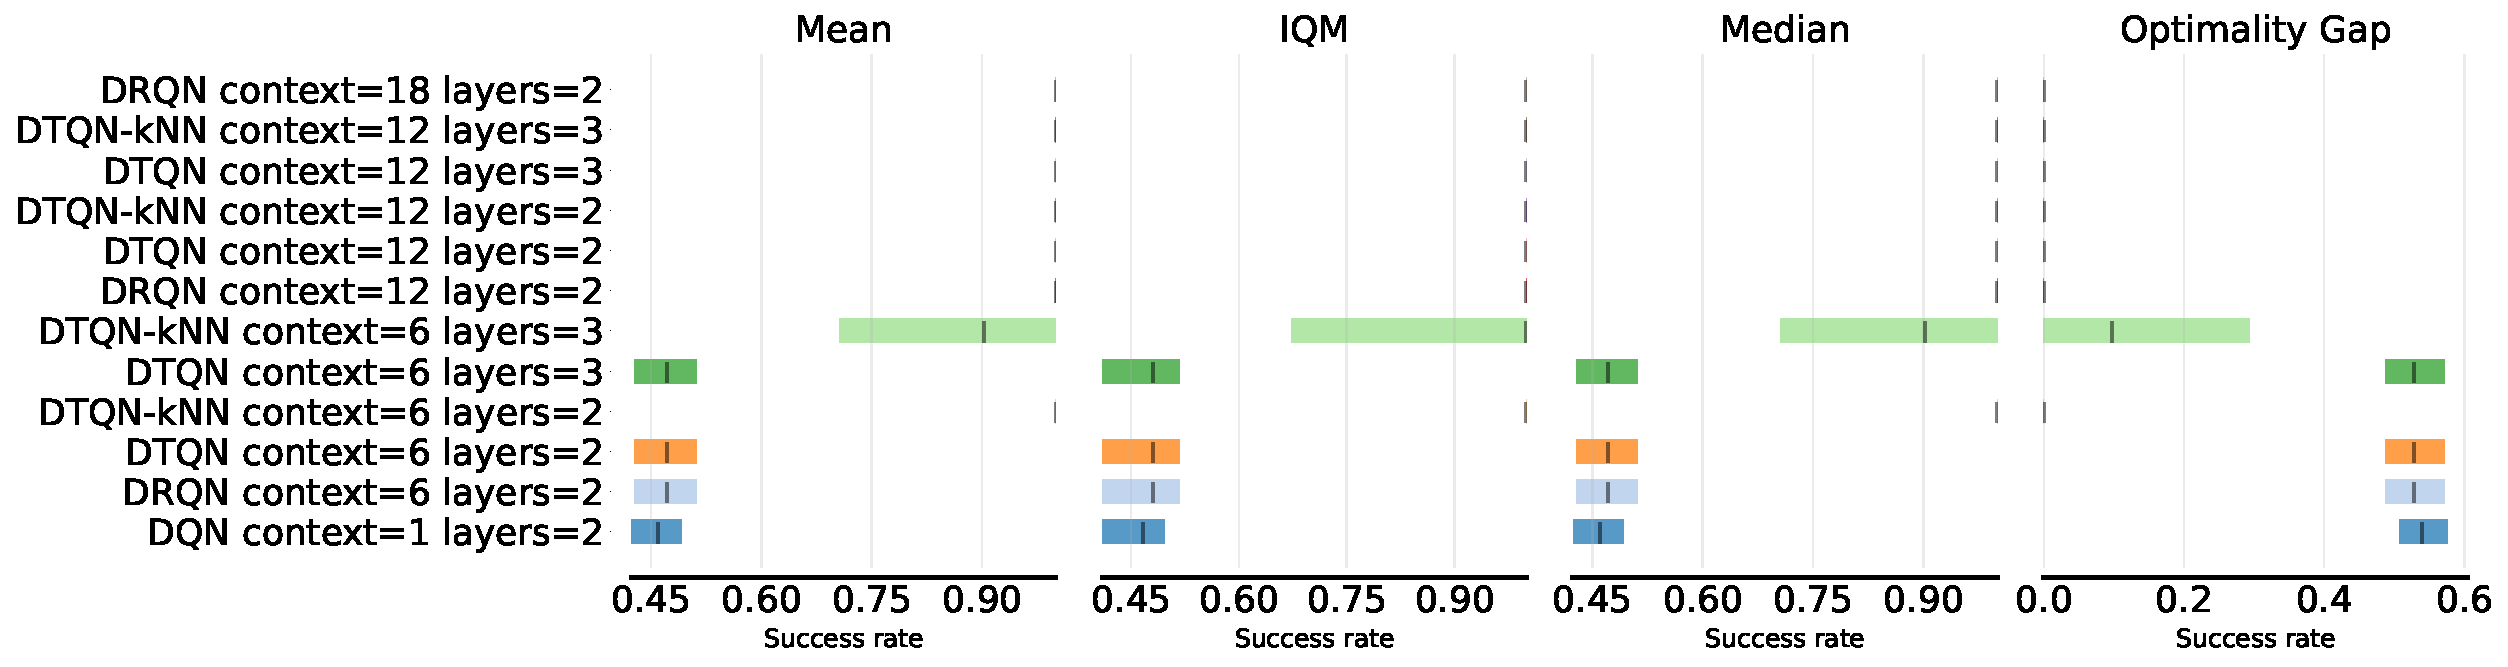
\includegraphics[width=\linewidth]{aggregate_metrics}
  \caption{Mean, interquartile mean (IQM), median and optimality gap of the final
    success rate, with 95\% stratified bootstrap confidence intervals.}
  \label{fig:aggregate-metrics}
\end{figure}

\begin{figure}[t]
  \centering
  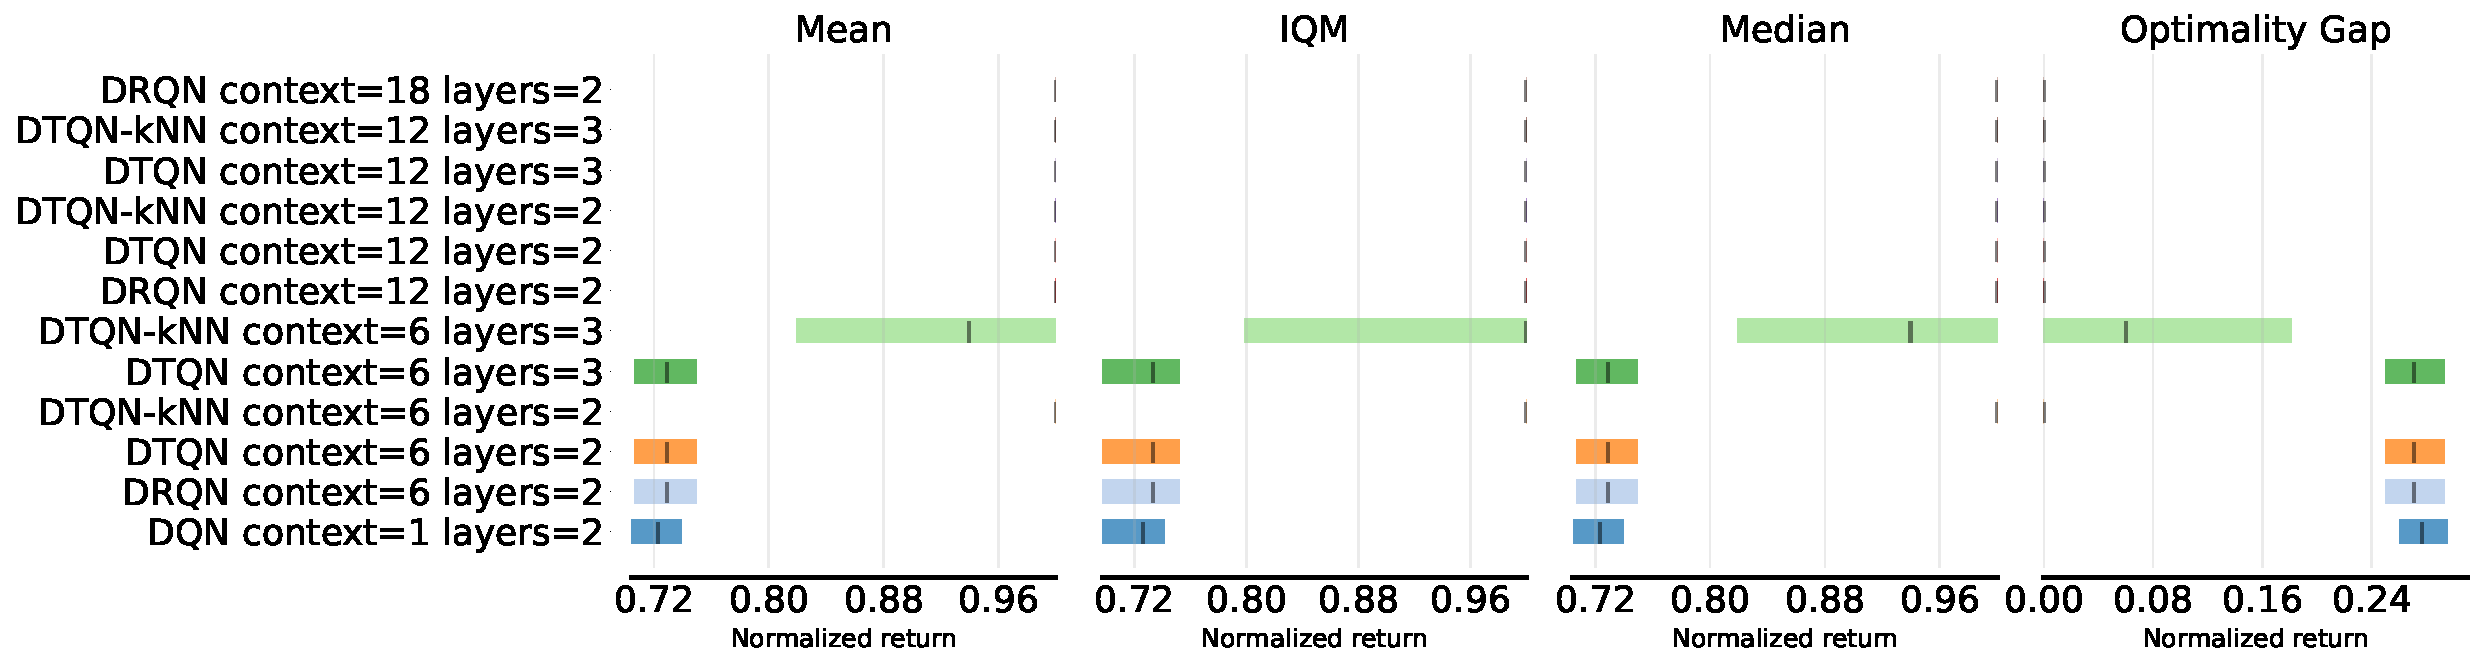
\includegraphics[width=\linewidth]{aggregate_metrics_return}
  \caption{Aggregate metrics of the final return, min-max normalized per task over
    all runs, with 95\% stratified bootstrap confidence intervals.}
  \label{fig:aggregate-metrics-return}
\end{figure}

\begin{figure}[t]
  \centering
  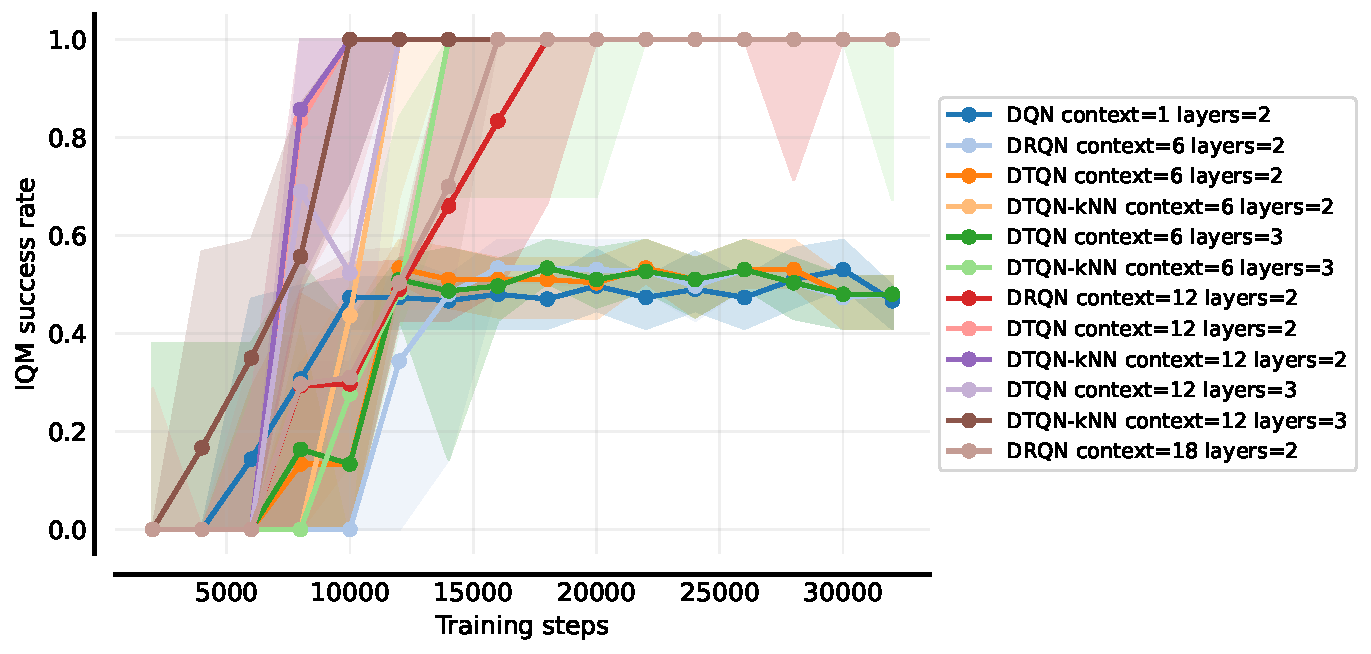
\includegraphics[width=\linewidth]{iqm_learning_curves}
  \caption{IQM success rate during training, with 95\% stratified bootstrap
    confidence bands.}
  \label{fig:iqm-learning-curves}
\end{figure}

\begin{figure}[t]
  \centering
  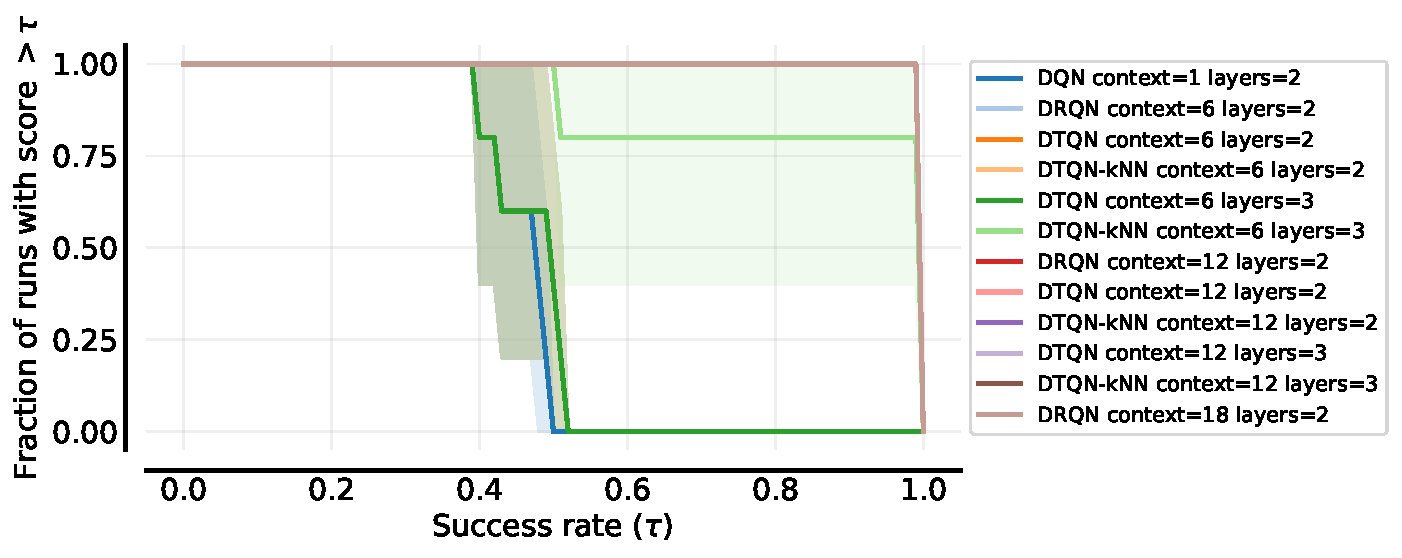
\includegraphics[width=\linewidth]{performance_profiles}
  \caption{Performance profiles: fraction of runs whose final success rate exceeds
    each threshold $\tau$, with 95\% confidence bands.}
  \label{fig:performance-profiles}
\end{figure}

\begin{figure}[t]
  \centering
  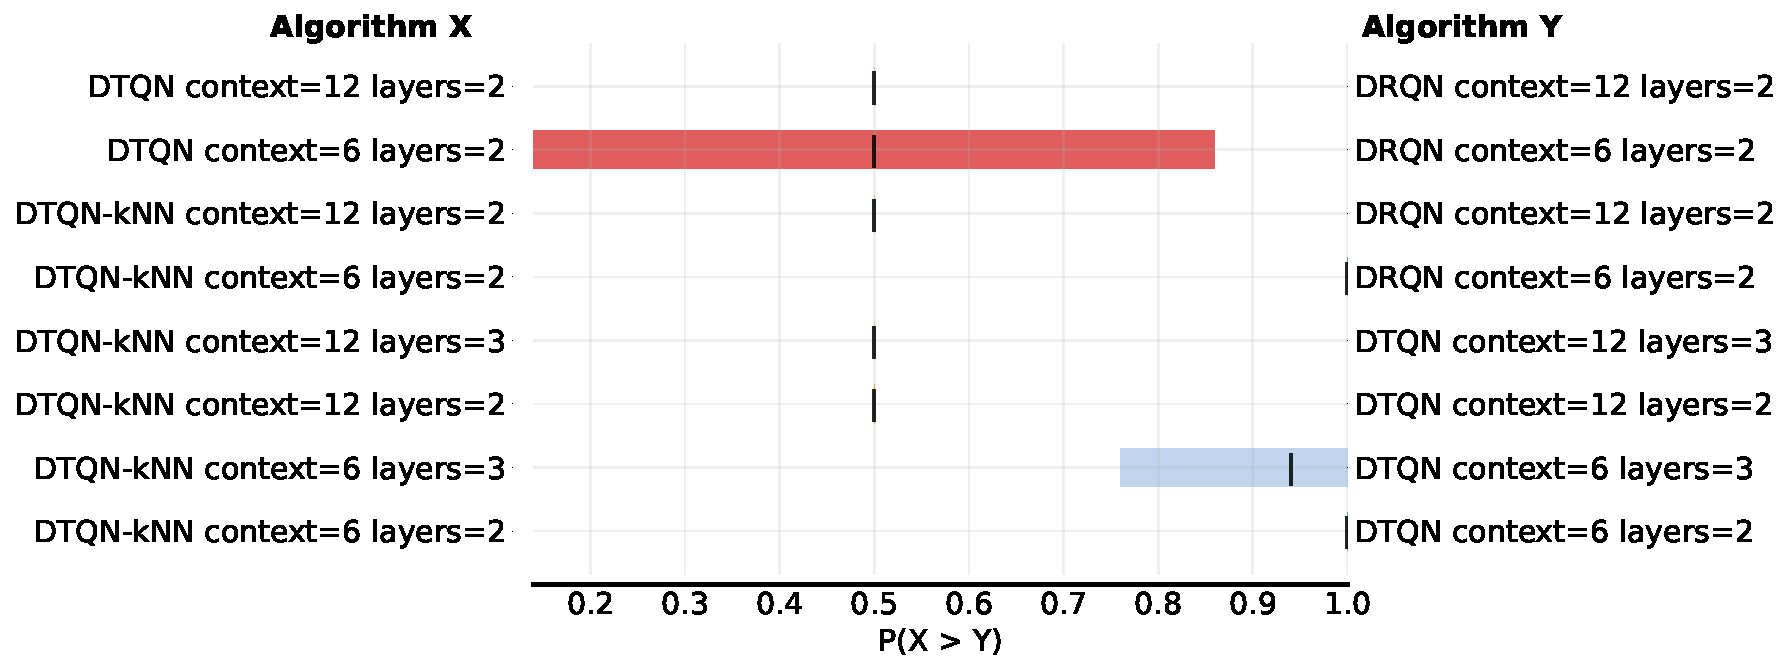
\includegraphics[width=0.8\linewidth]{probability_of_improvement}
  \caption{Probability of improvement of each candidate over its baseline with the
    same context length and number of layers, with 95\% confidence intervals.}
  \label{fig:probability-of-improvement}
\end{figure}

\section{Discussion}
\label{sec:discussion}
% TODO: Interpretation, limitations, threats to validity.
% refs: \cite{wu2022memorizing,dai2019transformerxl,parisotto2020gtrxl}

\section{Conclusion}
\label{sec:conclusion}
% TODO: Summary of contributions, findings and future work.


\bibliographystyle{unsrt}
\bibliography{references}

\end{document}
